\documentclass[10pt]{article}

\usepackage[margin=1in, letterpaper]{geometry}
\usepackage{parskip}

\usepackage{amsthm, amsmath, amssymb}
\usepackage{gensymb}  % For use of degree symbol
\usepackage[pdftex]{graphicx}
\usepackage{hyperref}

\usepackage{enumerate} % For use of (a), (b), et cetera
\usepackage{booktabs} % Tables
\usepackage[margin=20pt, labelfont=bf, labelsep=period,
justification=justified]{caption} % Captions in figure floats

% ======================
% Document setup, layout
% ======================

% The following metadata will show up in the PDF properties
\hypersetup{
	colorlinks = true,
	urlcolor = magenta,  % Links to URLs
	linkcolor = blue,  % Links within PDF
	pdfauthor = {Aaron Tran},
	pdfkeywords = {berkeley},
	pdftitle = {Astro 121, UG Radio Lab, Lab 4 - \today},
	pdfsubject = {},
	pdfpagemode = UseNone
}

% Don't indent paragraphs
\setlength\parindent{0em}

% Slightly more compact lines
\linespread{0.95}

% ===============
% Useful commands
% ===============
\newcommand {\mt}{\mathrm}
\newcommand {\unit}[1]{\; \mt{#1}}
% http://vemod.net/typesetting-units-in-latex

% Sets, operators
\newcommand {\ints}{\mathbb{Z}}
\newcommand {\ptl}{\partial}
\newcommand {\dl}{\nabla}

\begin{document}

% =======
% Titling
% =======
\begin{center}
\Large{Partial $1420\unit{MHz}$ HI Survey of the North Polar Spur}

\normalsize
\textbf{Aaron Tran}${}^{1,3}$ \\
Isaac A. Domagalski${}^{1,2}$, Caleb Levy${}^{1,2}$ \\
Aaron Parsons${}^{2,4,5}$, Garrett K. Keating${}^{2,4,5}$, Baylee Bordwell${}^{2,5}$ \\
\footnotesize
${}^1$Central Intelligence Agency, 1000 Colonial Farm Rd, McLean, VA 22101, USA \\
${}^2$Dept. Astronomy, UC Berkeley, D-23 Hearst Field Annex, Berkeley, CA 94720, USA \\
${}^3$Dept. Earth and Planetary Science, UC Berkeley, 335 McCone Hall, Berkeley, CA 94720, USA \\
${}^4$Radio Astronomy Laboratory, UC Berkeley, Berkeley, CA 94720, USA \\
${}^5$Undergraduate Radio Laboratory teaching staff \\
\textit{Submitted 2014 May ??}
\end{center}

% ========
% Abstract
% ========
\section*{Abstract}

We observe the north polar spur and stuff

% ============
% Introduction
% ============
\section{Introduction}

background on NPS.  Supernovae, snowploughs, shocks, Sedov, whatever.
ISM, physical properties inferrable.

% ============
% Observations
% ============
\section{Observations}

% ------------------------
% Leuschner specifications
% ------------------------
\subsection{Leuschner radio dish}

We use the Leuschner radio dish ($37\degree 55' 10.2'' \unit{N}$, $-122\degree 09' 12.4'' \unit{E}$), operated by UC Berkeley as part of Leuschner Observatory, to collect single-dish observations of the hyperfine HI line.  The Leuschner radio dish, hereafter Leuschner (Figure \ref{fig:kartp}), has diameter $3.6\unit{m}$ or $4.5\unit{m}$ depending on who is asked; the beamwidth is $\sim4\degree$ at its operating frequency of $1420 \unit{MHz}$.  Leuschner's view at low altitudes is blocked by surrounding hills; to the north Leuschner may point above $\sim50\degree$, to the south Leuschner may point to $20$--$30\degree$ altitude.  The Leuschner radio dish was built for the SETI Rapid Prototype Array (an early prototype for the now-underfunded and incomplete Allen Telescope Array); the dish has since been appropriated for undergraduate education.

\begin{figure}[!ht]
    \centering
    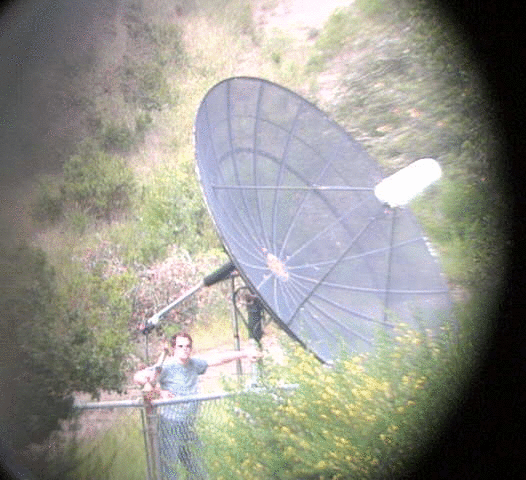
\includegraphics[width=0.5\textwidth]{kartp.png} \\
    \caption{The Leuschner dish has beamwidth $\sim 4 \degree$ at $1420 \unit{MHz}$.  Here the dish is shown with its erstwhile caretaker, \emph{kartp} (courtesy of I. Domagalski, E. Herrera, K. Moses).}
    \label{fig:kartp}
\end{figure}

RF waves incident on Leuschner are passed through a $200 \unit{MHz}$ bandpass filter centered on $1420 \unit{MHz}$ and mixed with a local oscillator (LO) signal of frequency $f_{\mt{LO}}$; both operations are performed at the antenna feed.  The LO mixing sends frequencies of interest near $1420 \unit{MHz}$ to $\sim150 \unit{MHz}$; this down-converted signal is routed to Leuschner Observatory facilities and bandpass filtered at $145$--$155 \unit{MHz}$.

The signal is digitized by an FPGA-based spectrometer using a polyphase filter bank; the effective sampling rate is $24 \unit{MHz}$ giving a bandwidth $144$--$156 \unit{MHz}$; the signal of interest appears in our frequency output via Nyquist aliasing [Siemion, 2012].  To characterize system temperature and frequency-dependent gain during data reduction, we collect observations at two LO frequencies $f_{\mt{LO}} = 1268.9 \unit{MHz}$ and $f_{\mt{LO}} = 1271.9 \unit{MHz}$.  The bandwidth $144$--$156 \unit{MHz}$ thus corresponds to the radio frequency bands $1412.9$--$1424.9 \unit{MHz}$ and $1415.9$--$1427.9 \unit{MHz}$ respectively.

% Observing campaign
\subsection{Observing campaign}

We observed the region of the sky with galactic latitude $b\geq 0\degree$ and galactic longitudes between $l=210\degree$ and $l=20\degree$, which contains the North Polar Spur.over the timespan of 2014 April 26 to 2014 May 5.

Unfortunately, blah was not visible from the interferometer during our observing campaign and could not be mapped.

In order to completely map the sky, the region of interest should be sampled with spacing $2\degree$ (for beamwidth $4\degree$).  In reality, hah.  We sampled most of the available region at $4\degree$ spacing.

BRIEFLY explain observing procedure, zig-zagging in lat/lon, criterion for point visibility as computed by Isaac (Check this yourself if there's time).

936 not visible?\\
1119 need data\\
444 we have data
total: ~2500

% ==============
% Data reduction
% ==============
\section{Data reduction}

\subsection{RFI removal}

Caleb's thing.  Remove spikes by taking min of 4 point bins.

\subsection{Calibration}

cf carl heiles' intensity handout
cool method.

Integration times were chosen so error would be nice (mainly for noise).  Integration time for main observations dictated by physical brightness temp.

\subsection{Image generation}

Due to a shortage of time, I did not finish my own
velocity computation etc... scripts.  Mainly needed baseline fitting/removal, peak identification.  (but, after baseline removal, I'd be able to get the main science done).  Working on it now would require branching Isaac's pipeline, and risk messing up the current data processing pipeline.  So I shan't do that yet...

Later on, I really want to be able to decompose the various peaks.  It
looks like our spur observations don't have multiple peaks anyways, so it's not
so bad since we don't care about the galactic plane.

% =======
% Results
% =======
\section{Results}

\begin{figure}[!ht]
    \centering
    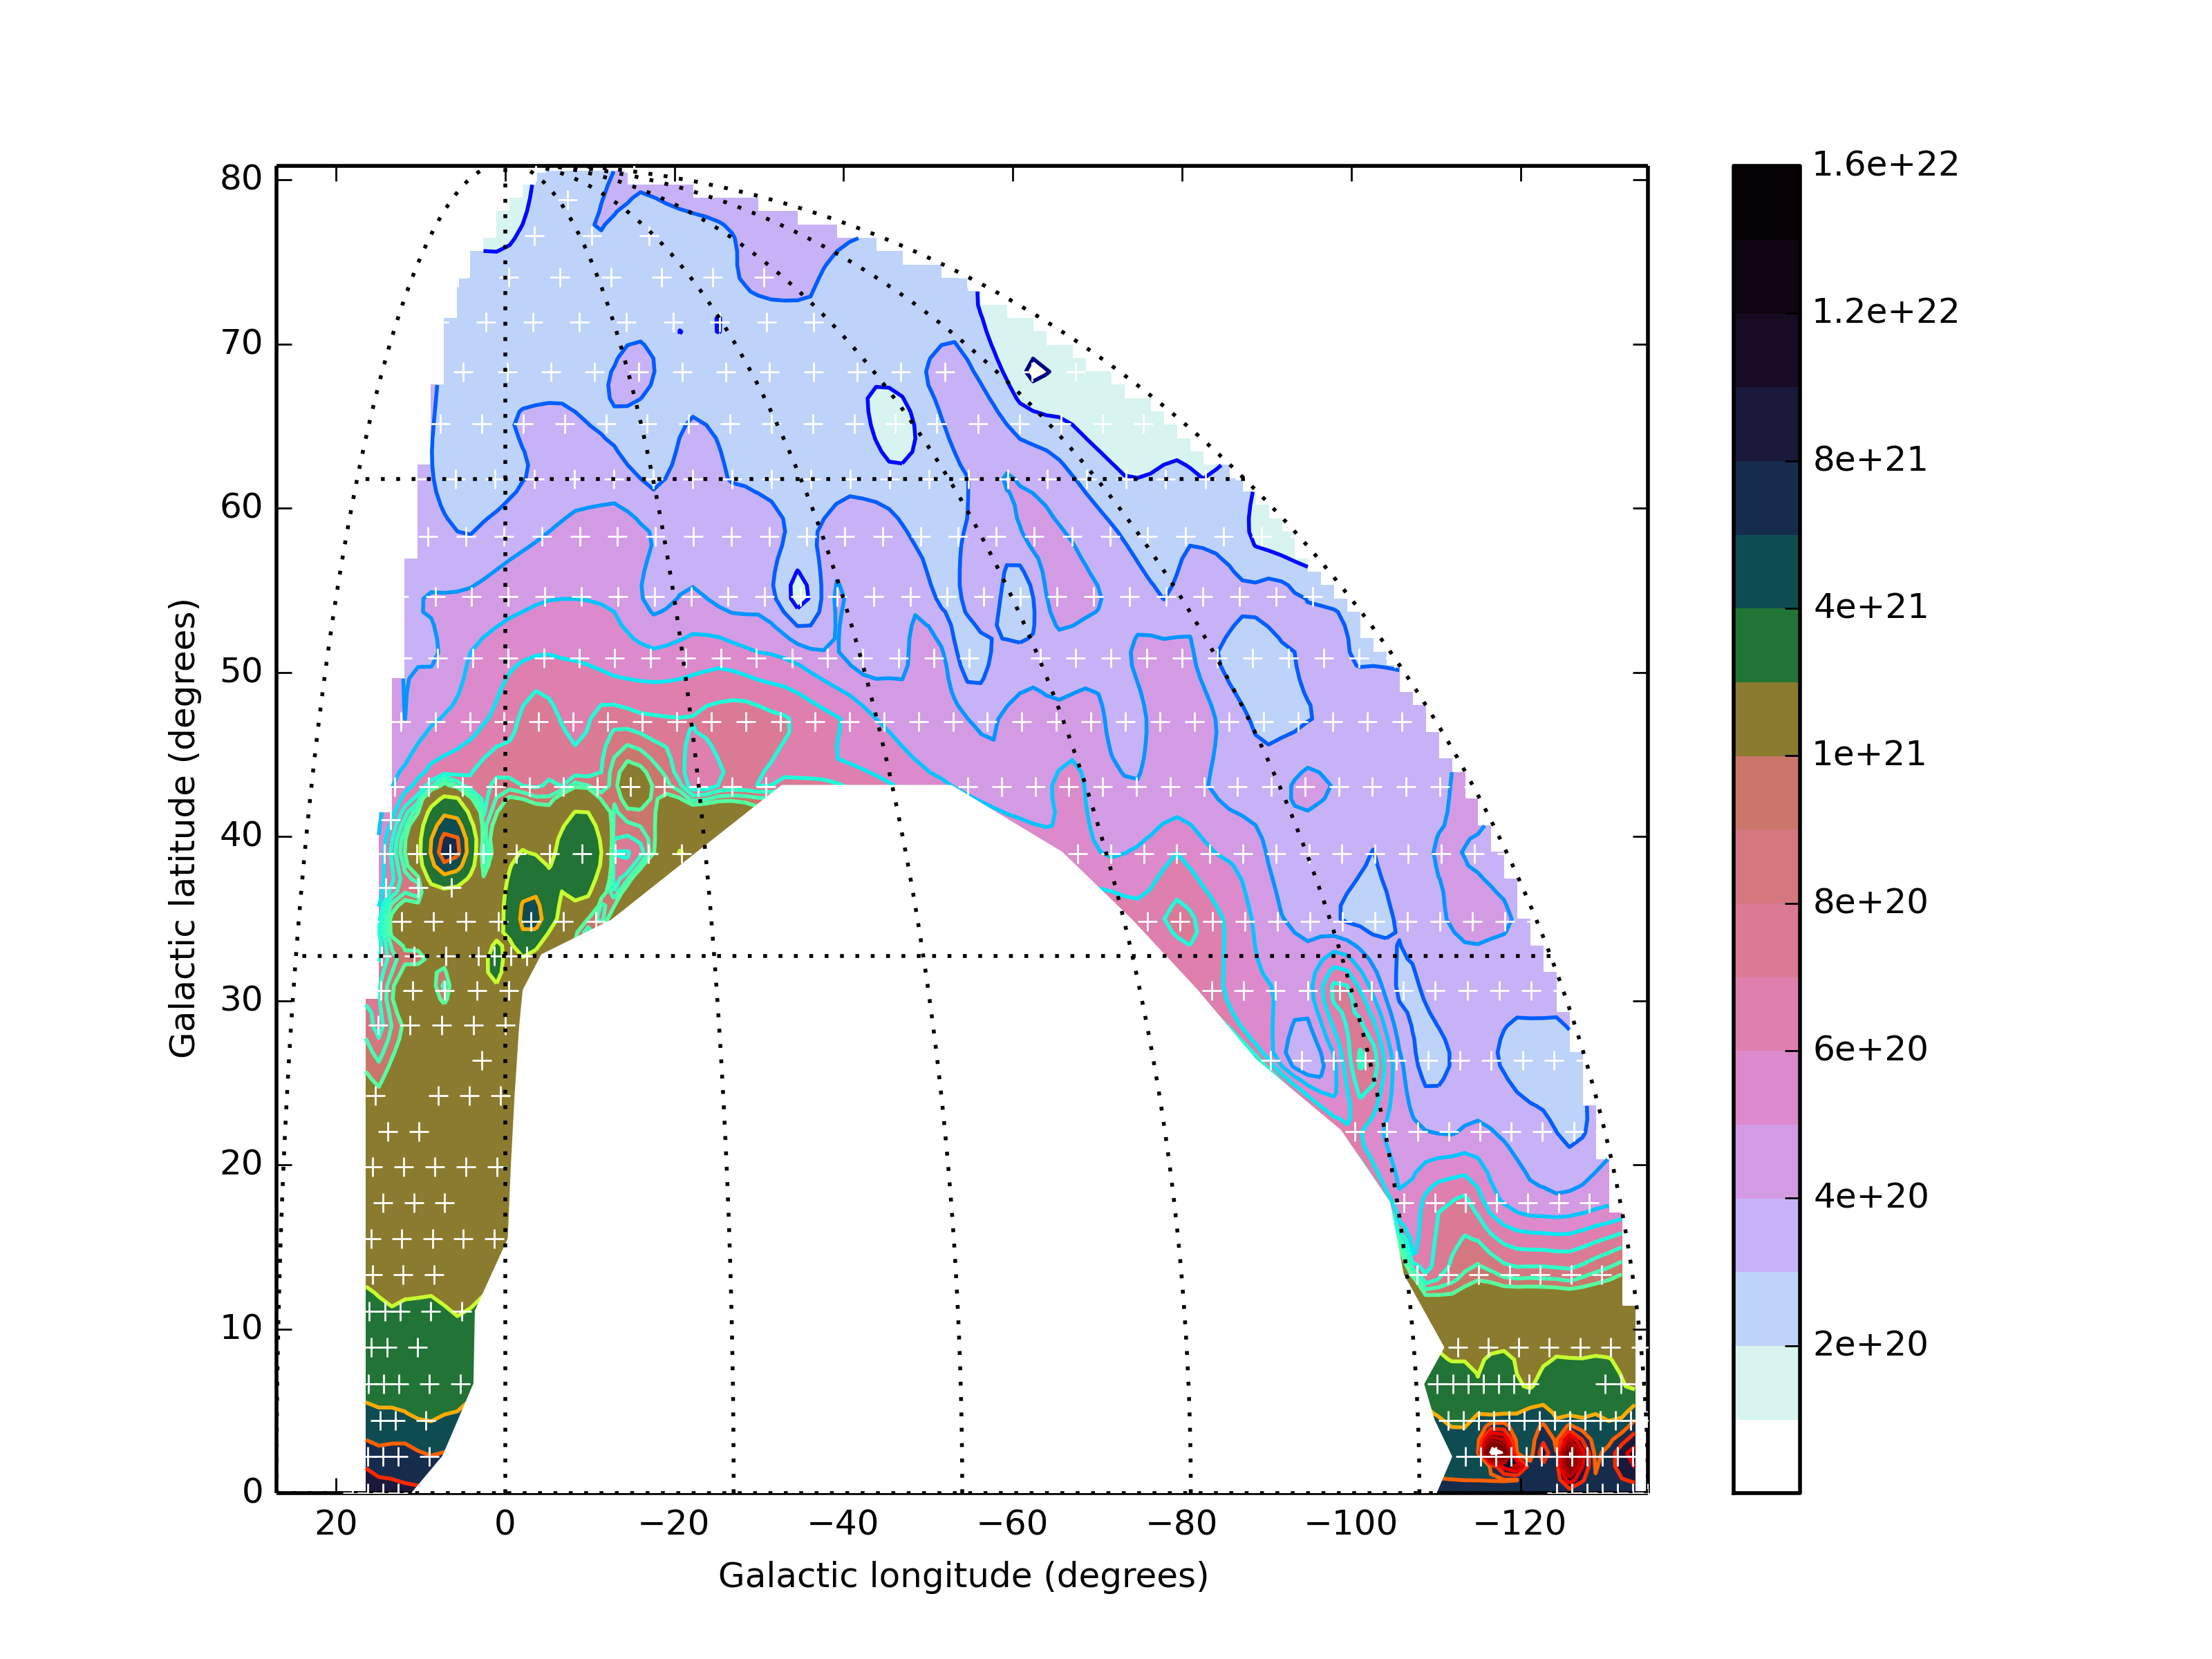
\includegraphics[width=0.5\textwidth]{plots/col_density.png} \\
    \caption{Column density}
    \label{fig:colrho}
\end{figure}
\begin{figure}[!ht]
    \centering
    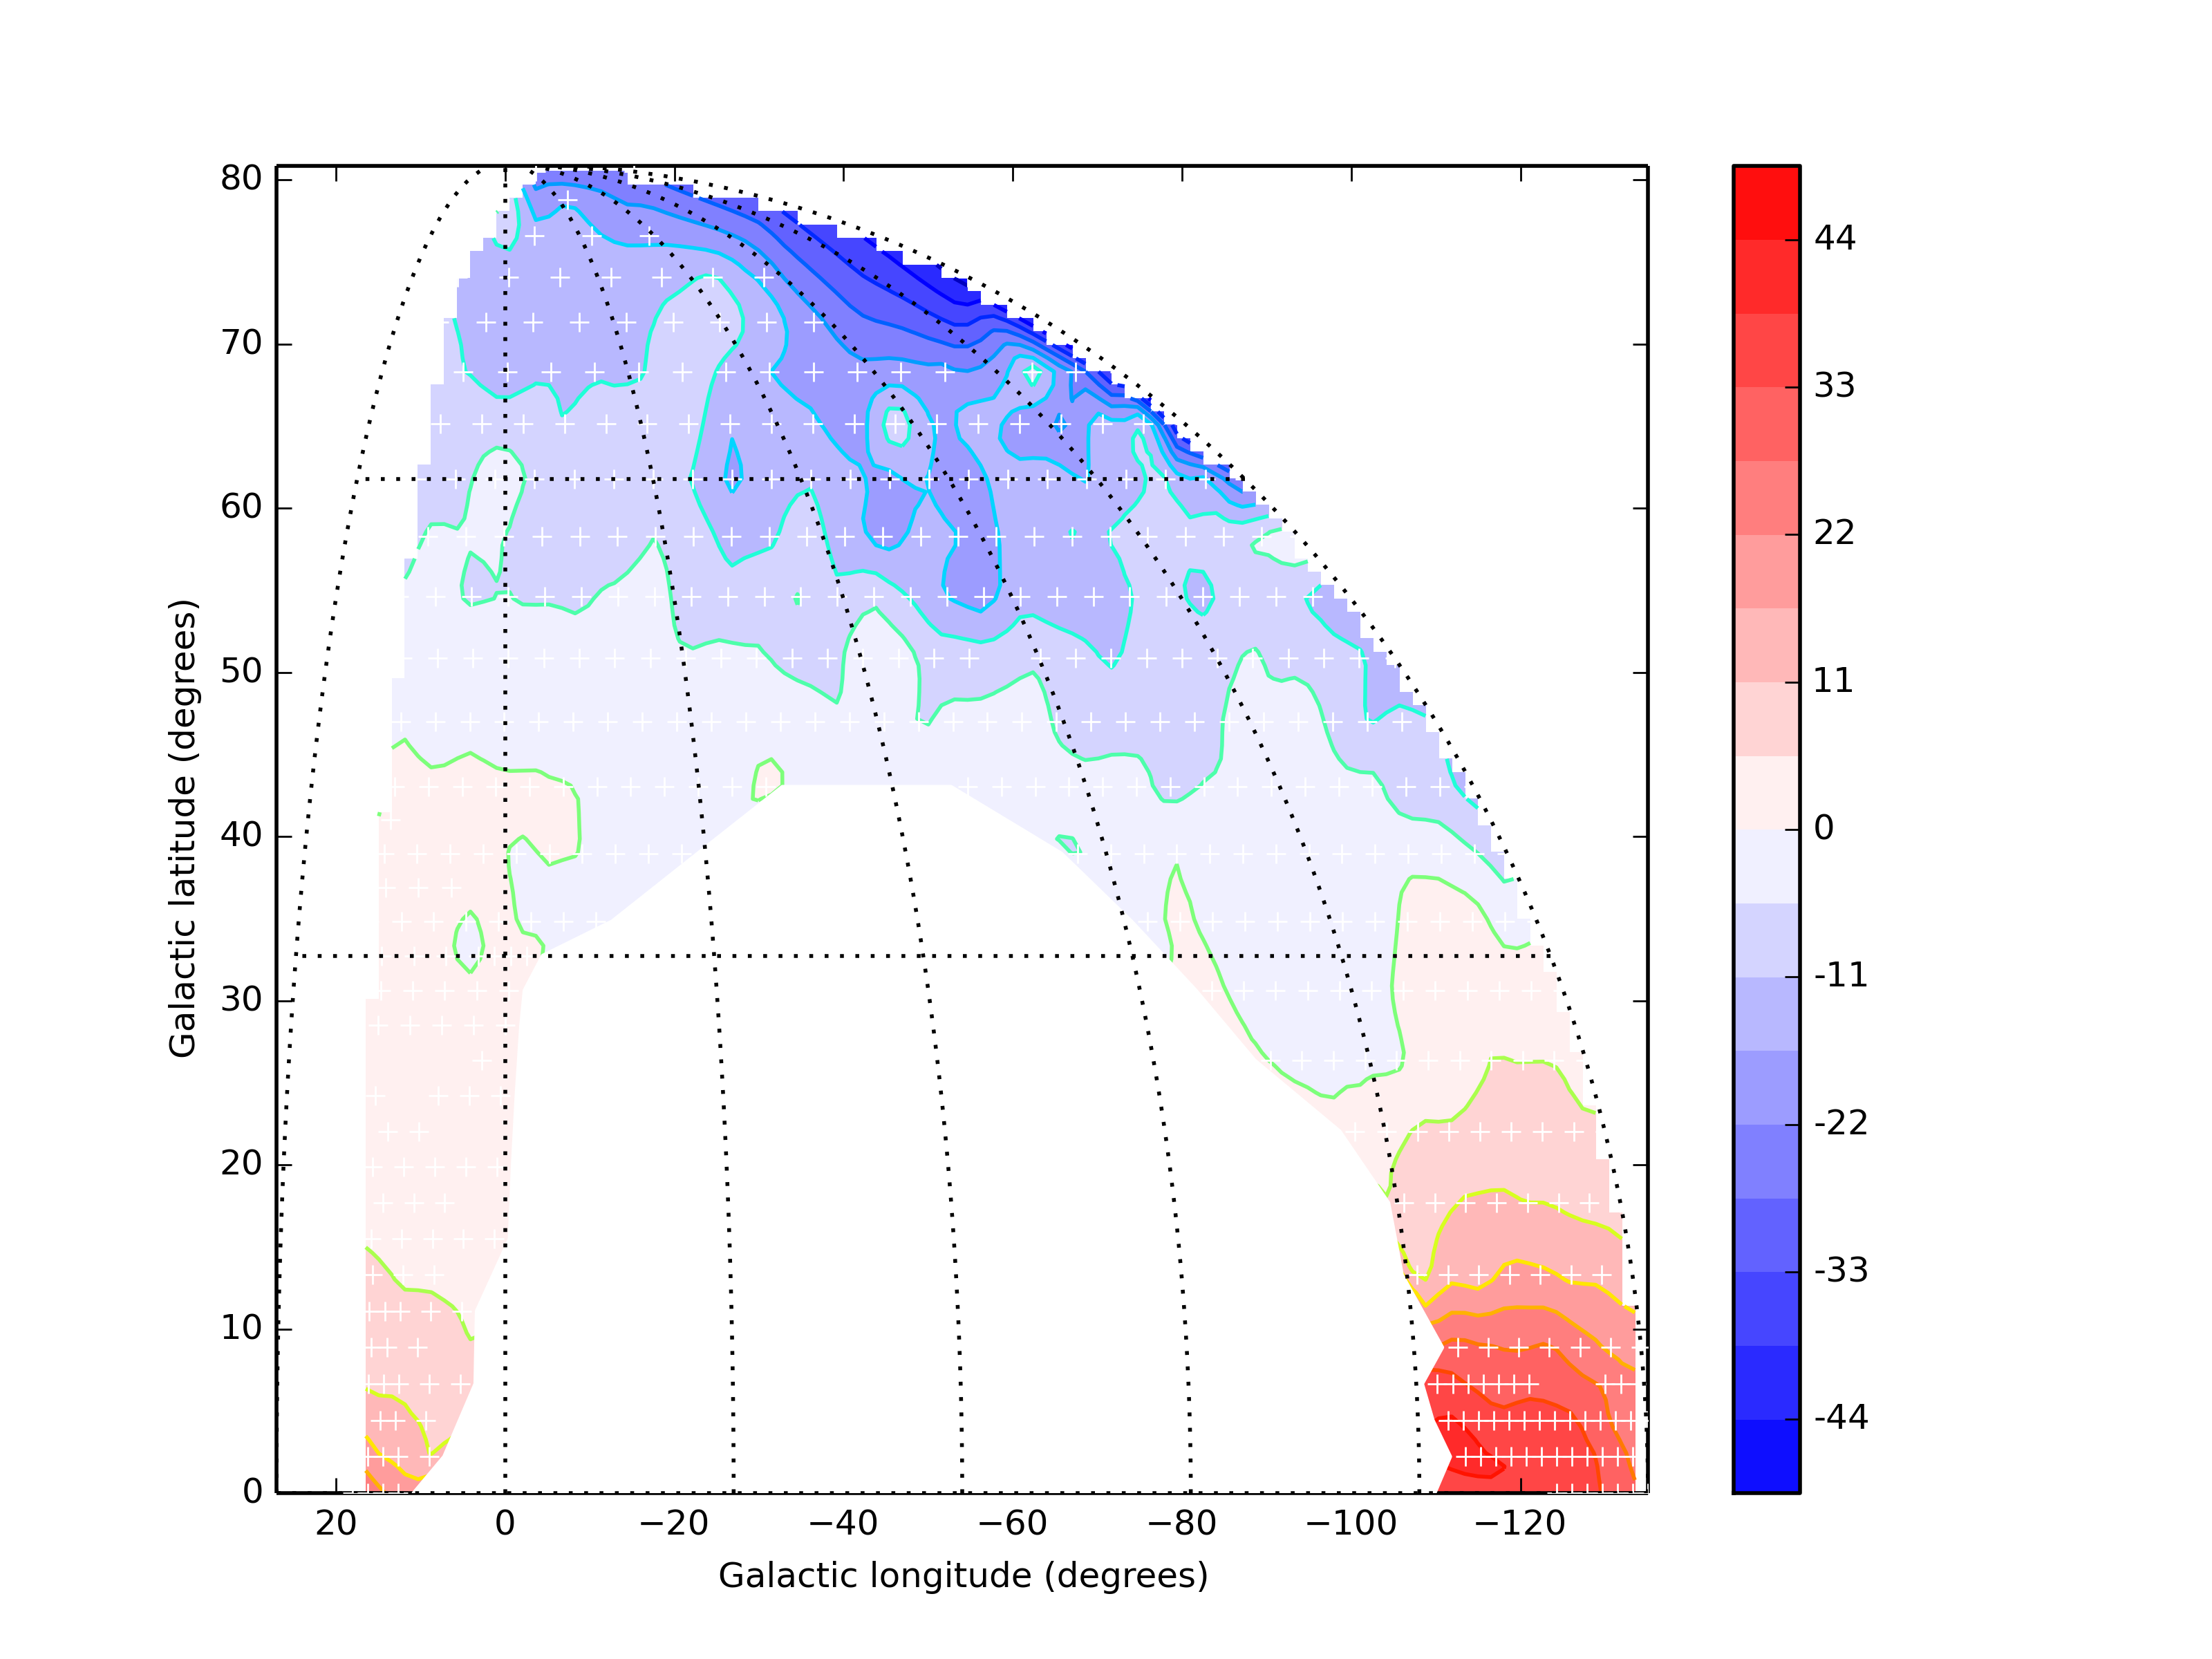
\includegraphics[width=0.48\textwidth]{plots/veloc_mean.png}
    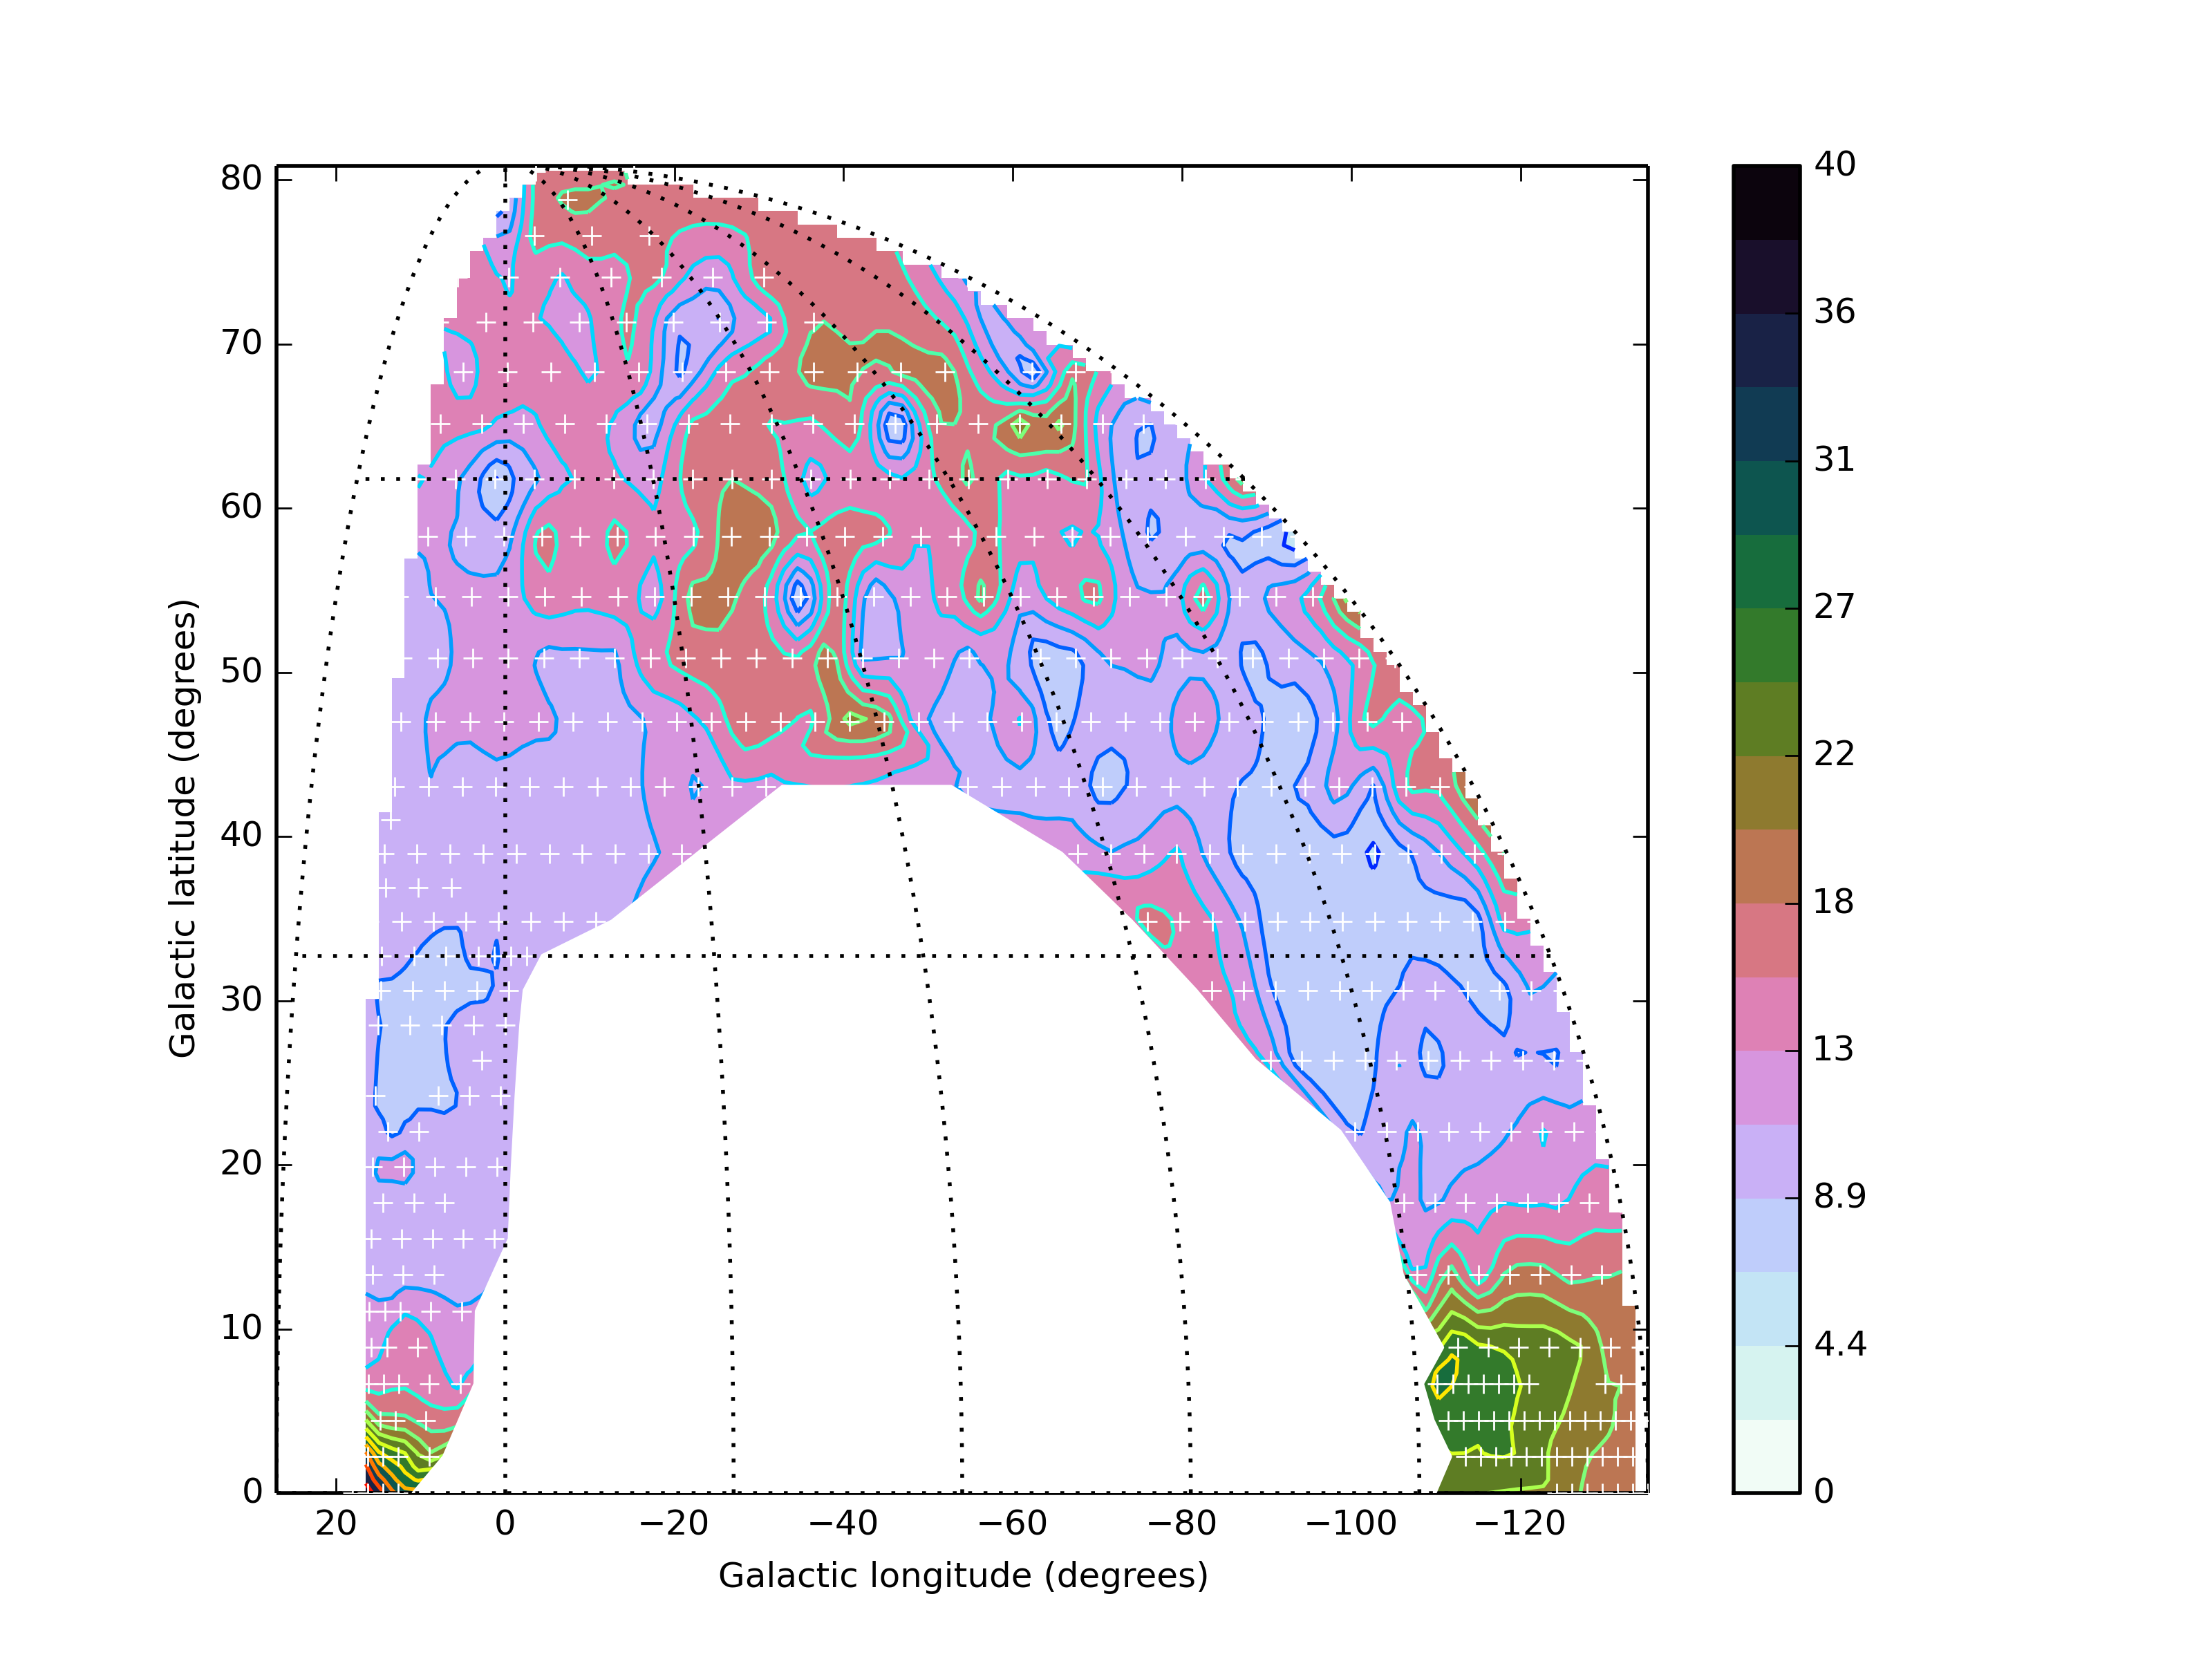
\includegraphics[width=0.48\textwidth]{plots/veloc_std.png} \\
    \caption{Mean velocity (left), stdev of velocity (right)}
    \label{fig:velocs}
\end{figure}

To dos...

(manual Mollweide projection + colorbars + zooming + better plots is partway done...)

completely overhaul images (manually compute mollweide projection and image\\ interpolation instead of relying on meshgrid)\\
include colorbars\\
determine physiologically sensible colormaps\\
determine best nonlinear colormapping\\
reduce pdf file sizes...

Here's a picture of work in progress.

\begin{figure}[!ht]
    \centering
    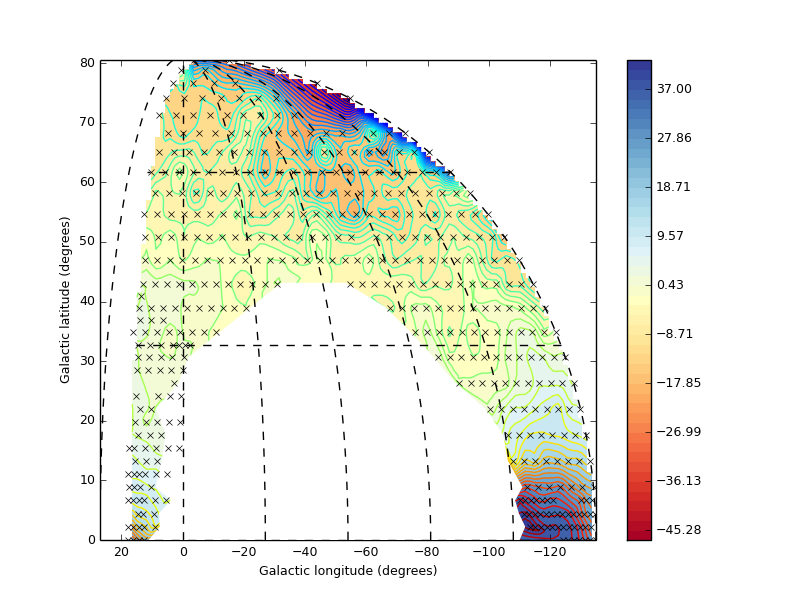
\includegraphics[width=0.48\textwidth]{v_ave_temporary.png}
    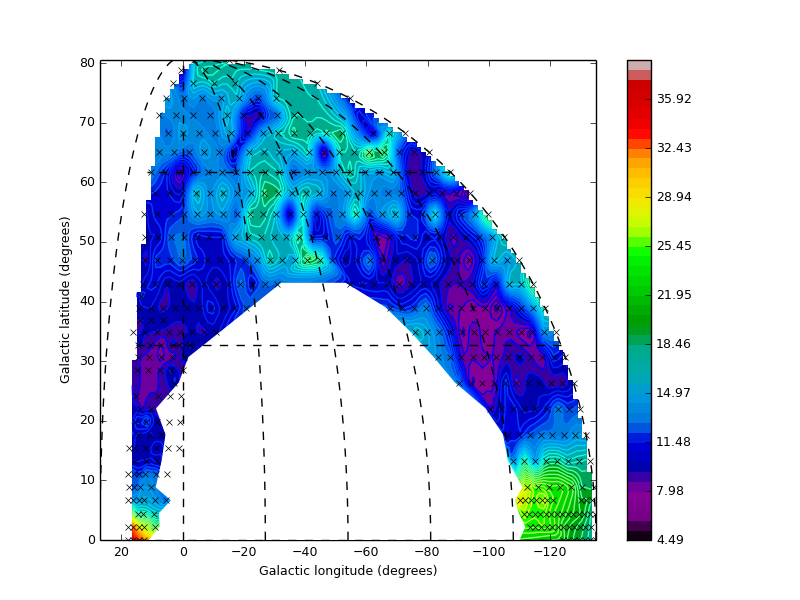
\includegraphics[width=0.48\textwidth]{v_std_temporary.png} \\
    \caption{Mean velocity (left), stdev of velocity (right).  Units are km/s for colors.}
    \label{fig:velocs_again}
\end{figure}

Comparing the dispersion to the velocity mean looks promising!  As we might expect, dispersion is stronger towards the center of our postulated/expected bubble, a more robust velocity signal is seen at edges.

The column density plot absolutely needs a logarithmic color scaling to see anything outside of the galactic plane.

% ==========
% Discussion
% ==========
\section{Discussion}

IF I separate out lines and get individual linewidths etc (by gaussian fit, dispersion for indiv peaks, however you like) -- start considering physical phenomena that give rise to broadening.

% ===========
% Conclusions
% ===========
\section{Conclusions}

\section{Acknowledgments}

\begin{figure}[!ht]
    \centering
    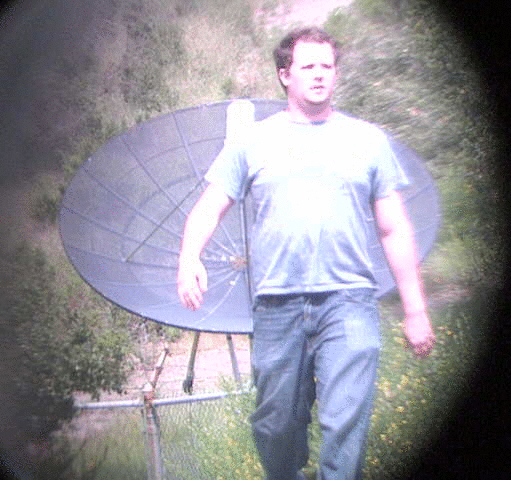
\includegraphics[width=0.5\textwidth]{kartp2.png} \\
    \caption{(image courtesy of I. Domagalski, E. Herrera, K. Moses)}
    \label{fig:kartp2}
\end{figure}

\begin{center}
Kartp noster, qui es in radiolab:\\
sanctificetur nomen tuum;\\
adveniat regnum tuum;\\
fiat voluntas tua.\\
sicut in academia, et in universitas.\\
Observationem nostrum cotidianum da nobis hodie;\\
et dimitte nobis errores nostra,\\
sicut et nos dimittimus erroribus nostris;\\
et ne nos inducas in tentationem;\\
sed libera nos a circumsonum.
\end{center}

%Karto and Baylee are gr8.
%Isaac and Caleb are gr8.
%Aaron Parsons is cool.

\section{Author contributions}

I. A. D. did stuff.  C. L. did stuff.  A. T. did stuff.

\section{Electronic supplement}

All supporting files are stored on the repository:\\
\href{https://github.com/aarontran/ay121}
{https://github.com/aarontran/ay121/lab4/}.

\section{References}

\hangindent 0.25in Condon, J. J. and S. M. Ransom (2006), Essential Radio Astronomy, \\
\href{http://www.cv.nrao.edu/course/astr534/ERA.shtml}
{http://www.cv.nrao.edu/course/astr534/ERA.shtml}.

\hangindent 0.25in Green, R. M. (1985), \textit{Spherical astronomy}, 520pp.,
Cambridge Univ. Press, Cambridge.

\hangindent 0.25in Siemion, A. (2012), Leuschner Spectrometer, CASPER documentation wiki, \\
\href{https://casper.berkeley.edu/wiki/Leuschner\_Spectrometer}
{https://casper.berkeley.edu/wiki/Leuschner\_Spectrometer}.

\hangindent 0.25in Wolleben, M. (2007), A New Model for the Loop I (North Polar
Spur) Region, \textit{Astrophys. J.}, \textit{664}, 349--356,
doi:10.1086/518711.

\end{document}
